% Options for packages loaded elsewhere
\PassOptionsToPackage{unicode}{hyperref}
\PassOptionsToPackage{hyphens}{url}
%
\documentclass[
]{book}
\usepackage{lmodern}
\usepackage{amssymb,amsmath}
\usepackage{ifxetex,ifluatex}
\ifnum 0\ifxetex 1\fi\ifluatex 1\fi=0 % if pdftex
  \usepackage[T1]{fontenc}
  \usepackage[utf8]{inputenc}
  \usepackage{textcomp} % provide euro and other symbols
\else % if luatex or xetex
  \usepackage{unicode-math}
  \defaultfontfeatures{Scale=MatchLowercase}
  \defaultfontfeatures[\rmfamily]{Ligatures=TeX,Scale=1}
\fi
% Use upquote if available, for straight quotes in verbatim environments
\IfFileExists{upquote.sty}{\usepackage{upquote}}{}
\IfFileExists{microtype.sty}{% use microtype if available
  \usepackage[]{microtype}
  \UseMicrotypeSet[protrusion]{basicmath} % disable protrusion for tt fonts
}{}
\makeatletter
\@ifundefined{KOMAClassName}{% if non-KOMA class
  \IfFileExists{parskip.sty}{%
    \usepackage{parskip}
  }{% else
    \setlength{\parindent}{0pt}
    \setlength{\parskip}{6pt plus 2pt minus 1pt}}
}{% if KOMA class
  \KOMAoptions{parskip=half}}
\makeatother
\usepackage{xcolor}
\IfFileExists{xurl.sty}{\usepackage{xurl}}{} % add URL line breaks if available
\IfFileExists{bookmark.sty}{\usepackage{bookmark}}{\usepackage{hyperref}}
\hypersetup{
  pdftitle={Guide for Wise Investing},
  pdfauthor={Junghoon Shin},
  hidelinks,
  pdfcreator={LaTeX via pandoc}}
\urlstyle{same} % disable monospaced font for URLs
\usepackage{longtable,booktabs}
% Correct order of tables after \paragraph or \subparagraph
\usepackage{etoolbox}
\makeatletter
\patchcmd\longtable{\par}{\if@noskipsec\mbox{}\fi\par}{}{}
\makeatother
% Allow footnotes in longtable head/foot
\IfFileExists{footnotehyper.sty}{\usepackage{footnotehyper}}{\usepackage{footnote}}
\makesavenoteenv{longtable}
\usepackage{graphicx,grffile}
\makeatletter
\def\maxwidth{\ifdim\Gin@nat@width>\linewidth\linewidth\else\Gin@nat@width\fi}
\def\maxheight{\ifdim\Gin@nat@height>\textheight\textheight\else\Gin@nat@height\fi}
\makeatother
% Scale images if necessary, so that they will not overflow the page
% margins by default, and it is still possible to overwrite the defaults
% using explicit options in \includegraphics[width, height, ...]{}
\setkeys{Gin}{width=\maxwidth,height=\maxheight,keepaspectratio}
% Set default figure placement to htbp
\makeatletter
\def\fps@figure{htbp}
\makeatother
\setlength{\emergencystretch}{3em} % prevent overfull lines
\providecommand{\tightlist}{%
  \setlength{\itemsep}{0pt}\setlength{\parskip}{0pt}}
\setcounter{secnumdepth}{5}
\usepackage{booktabs}
\usepackage{booktabs}
\usepackage{longtable}
\usepackage{array}
\usepackage{multirow}
\usepackage{wrapfig}
\usepackage{float}
\usepackage{colortbl}
\usepackage{pdflscape}
\usepackage{tabu}
\usepackage{threeparttable}
\usepackage{threeparttablex}
\usepackage[normalem]{ulem}
\usepackage{makecell}
\usepackage{xcolor}
\usepackage[]{natbib}
\bibliographystyle{apalike}

\title{Guide for Wise Investing}
\author{Junghoon Shin}
\date{2021-01-26 01:48:58 KST}

\begin{document}
\maketitle

{
\setcounter{tocdepth}{1}
\tableofcontents
}
\hypertarget{about-the-author}{%
\chapter*{About the author}\label{about-the-author}}
\addcontentsline{toc}{chapter}{About the author}

\href{mailto:junghoonshin@kaist.ac.kr}{\nolinkurl{junghoonshin@kaist.ac.kr}}

\hypertarget{part-part-i}{%
\part{Part I}\label{part-part-i}}

\hypertarget{buffett}{%
\chapter[Buffett's wisdom]{\texorpdfstring{Buffett's wisdom\footnote{The quotes are picked from \url{https://www.fool.com/investing/best-warren-buffett-quotes.aspx} and reorganized.}}{Buffett's wisdom}}\label{buffett}}

\begin{figure}
\centering
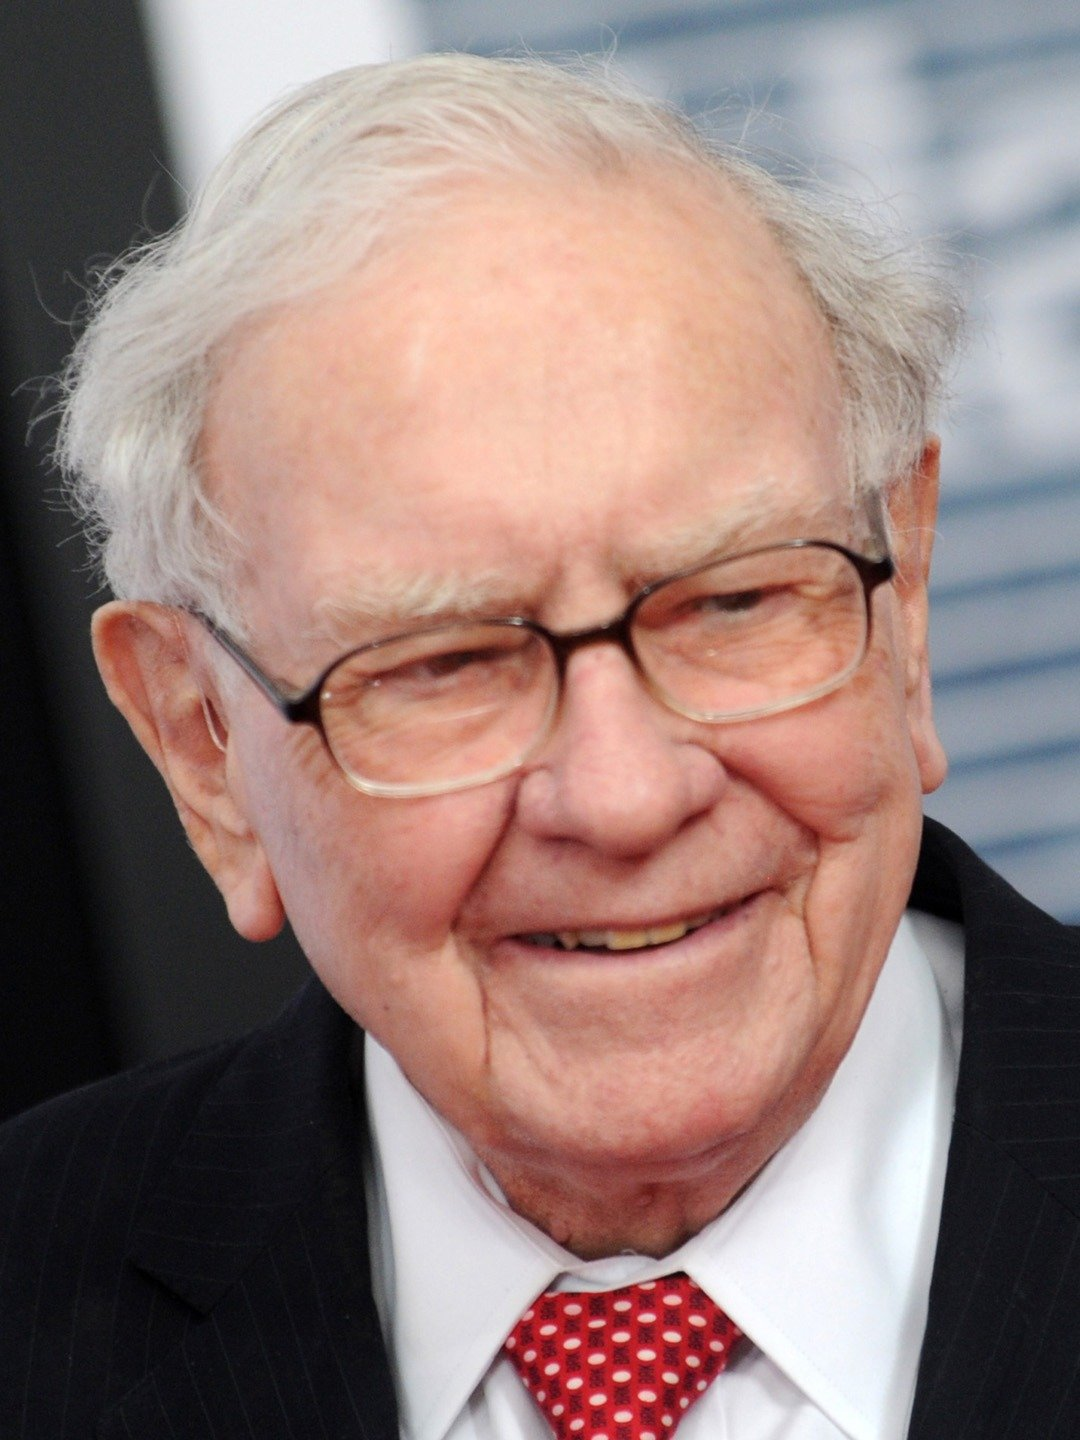
\includegraphics[width=2.5in,height=\textheight]{images/Warren.jpg}
\caption{Warren Buffet, CEO of Berkshire Hathaway}
\end{figure}

\hypertarget{rule-no.-1}{%
\section{Rule No.~1}\label{rule-no.-1}}

\begin{itemize}
\tightlist
\item
  ``Rule No.~1 is never lose money. Rule No.~2 is never forget Rule No.~1.''
\end{itemize}

\hypertarget{value-investing}{%
\section{Value investing}\label{value-investing}}

\begin{itemize}
\item
  ``Price is what you pay. Value is what you get.''
\item
  ``It's far better to buy a wonderful company at a fair price than a fair company at a wonderful price.''
\item
  ``The key to investing is not assessing how much an industry is going to affect society, or how much it will grow, but rather determining the competitive advantage of any given company and, above all, the durability of that advantage.''
\item
  ``Buy into a company because you want to own it, not because you want the stock to go up.''
\item
  ``Buy a stock the way you would buy a house. Understand and like it such that you'd be content to own it in the absence of any market.''
\end{itemize}

\hypertarget{investing-for-the-long-term}{%
\section{Investing for the long term}\label{investing-for-the-long-term}}

\begin{itemize}
\item
  ``Someone's sitting in the shade today because someone planted a tree a long time ago.''
\item
  ``If you aren't willing to own a stock for ten years, don't even think about owning it for ten minutes.''
\item
  ``All there is to investing is picking good stocks at good times and staying with them as long as they remain good companies.''
\item
  ``Do not take yearly results too seriously. Instead, focus on four or five-year averages.''
\end{itemize}

\hypertarget{dealing-with-losing-investments}{%
\section{Dealing with losing investments}\label{dealing-with-losing-investments}}

\begin{itemize}
\tightlist
\item
  ``The most important thing to do if you find yourself in a hole is to stop digging.''
\end{itemize}

\hypertarget{right-mindset-for-investing}{%
\section{Right mindset for investing}\label{right-mindset-for-investing}}

\begin{itemize}
\item
  ``We simply attempt to be fearful when others are greedy and to be greedy only when others are fearful.''
\item
  ``The most important quality for an investor is temperament, not intellect. You need a temperament that neither derives great pleasure from being with the crowd or against the crowd.''
\item
  ``It is not necessary to do extraordinary things to get extraordinary results.''
\item
  ``The difference between successful people and really successful people is that really successful people say no to almost everything.''
\end{itemize}

\hypertarget{market-crashes-and-recessions}{%
\section{Market crashes and recessions}\label{market-crashes-and-recessions}}

\begin{itemize}
\item
  ``In the 20th century, the United States endured two world wars and other traumatic and expensive military conflicts; the Depression; a dozen or so recessions and financial panics; oil shocks; a flu epidemic; and the resignation of a disgraced president. Yet the Dow rose from 66 to 11,497.''
\item
  ``Only when the tide goes out do you discover who's been swimming naked.''
\item
  ``Predicting rain doesn't count, building the ark does.''
\end{itemize}

\hypertarget{importance-of-learning}{%
\section{Importance of learning}\label{importance-of-learning}}

\begin{itemize}
\item
  ``Read 500 pages like this every day. That's how knowledge works. It builds up, like compound interest. All of you can do it, but I guarantee not many of you will do it.''
\item
  ``Never invest in a business you cannot understand.''
\item
  ``Risk comes from not knowing what you're doing.''
\end{itemize}

\hypertarget{ignoring-market-noise}{%
\section{Ignoring market noise}\label{ignoring-market-noise}}

\begin{itemize}
\item
  ``You are neither right nor wrong because the crowd disagrees with you. You are right because your data and reasoning are right.''
\item
  ``We've long felt that the only value of stock forecasters is to make fortune tellers look good. Even now, Charlie and I continue to believe that short-term market forecasts are poison and should be kept locked up in a safe place, away from children and also from grown-ups who behave in the market like children.''
\item
  ``Don't get caught up with what other people are doing. Being a contrarian isn't the key but being a crowd follower isn't either. You need to detach yourself emotionally.''
\end{itemize}

\hypertarget{indes-funds}{%
\section{Indes funds}\label{indes-funds}}

\begin{itemize}
\item
  ``Among the various propositions offered to you, if you invested in a very low cost index fund -- where you don't put the money in at one time, but average in over 10 years -- you'll do better than 90\% of people who start investing at the same time.''
\item
  ``Just pick a broad index like the S\&P 500. Don't put your money in all at once; do it over a period of time.''
\end{itemize}

\hypertarget{part-part-ii}{%
\part{Part II}\label{part-part-ii}}

\hypertarget{business}{%
\chapter{Business evaluation}\label{business}}

\hypertarget{comprehensive-financials}{%
\section[Comprehensive financials]{\texorpdfstring{Comprehensive financials\footnote{Data are from \href{https://www.google.com/finance}{Google Finance} and \href{https://finance.yahoo.com/}{Yahoo Finance}.}}{Comprehensive financials}}\label{comprehensive-financials}}

\includegraphics[width=1\linewidth]{guide-for-wise-investing_files/figure-latex/unnamed-chunk-5-1}\\
Adjusted Graham formula: as defined \href{https://www.oldschoolvalue.com/stock-valuation/benjamin-graham-formula/}{here}\\
BVPS: book value per share\\
DCF10: discounted cash flow in 10 years as defined \href{https://www.investopedia.com/terms/d/dcf.asp}{here}\\
EPS: earnings per share\\
High52: 52-week high price\\
Industry PER: data from \href{http://pages.stern.nyu.edu/~adamodar/New_Home_Page/datafile/pedata.html}{here}\\
Low52: 52-week low price\\
PBR: price/book value ratio\\
PEG: price/earnings-to-growth ratio\\
PER: price/earnings ratio\\
PSR: price/sales ratio\\
ROA: return on asset\\
ROE: return on equity\\
Sustainable growth rate: ROE \(\times\) retention ratio

\hypertarget{key-financials}{%
\section{Key financials}\label{key-financials}}

\begin{figure}

\includegraphics[width=1\linewidth]{guide-for-wise-investing_files/figure-latex/financials-figure-1} \caption{Key financials of my watchlist}\label{fig:financials-figure}
\end{figure}

\hypertarget{investing-decision}{%
\section[Investing decision]{\texorpdfstring{Investing decision\footnote{The value of a company in its early stage of development with zero or negative earnings cannot be determined based on its financials, but rather should be based on the subject matter knowledge about its mission, technologies, management and culture, as well as the industry overall.}}{Investing decision}}\label{investing-decision}}

\begin{figure}

\includegraphics[width=1\linewidth]{guide-for-wise-investing_files/figure-latex/unnamed-chunk-7-1} \caption{Investing decision made by a fundamental analysis-based algorithm for listed companies}\label{fig:unnamed-chunk-7}
\end{figure}

\hypertarget{stock-price-trend}{%
\section[Stock price trend]{\texorpdfstring{Stock price trend\footnote{All prices are normalized to 100 as of 2020-09-21.}}{Stock price trend}}\label{stock-price-trend}}

\begin{figure}

\includegraphics[width=1\linewidth]{guide-for-wise-investing_files/figure-latex/unnamed-chunk-9-1} \caption{Semiconductor}\label{fig:unnamed-chunk-9}
\end{figure}

\begin{figure}

\includegraphics[width=1\linewidth]{guide-for-wise-investing_files/figure-latex/unnamed-chunk-10-1} \caption{Drugs (Pharmaceutical)}\label{fig:unnamed-chunk-10}
\end{figure}

\begin{figure}

\includegraphics[width=1\linewidth]{guide-for-wise-investing_files/figure-latex/unnamed-chunk-11-1} \caption{Computers/Peripherals}\label{fig:unnamed-chunk-11}
\end{figure}

\begin{figure}

\includegraphics[width=1\linewidth]{guide-for-wise-investing_files/figure-latex/unnamed-chunk-12-1} \caption{Heathcare Information and Technology}\label{fig:unnamed-chunk-12}
\end{figure}

\begin{figure}

\includegraphics[width=1\linewidth]{guide-for-wise-investing_files/figure-latex/unnamed-chunk-13-1} \caption{Software (Entertainment)}\label{fig:unnamed-chunk-13}
\end{figure}

\begin{figure}

\includegraphics[width=1\linewidth]{guide-for-wise-investing_files/figure-latex/unnamed-chunk-14-1} \caption{Aerospace/Defense}\label{fig:unnamed-chunk-14}
\end{figure}

\begin{figure}

\includegraphics[width=1\linewidth]{guide-for-wise-investing_files/figure-latex/unnamed-chunk-15-1} \caption{Auto and Truck}\label{fig:unnamed-chunk-15}
\end{figure}

\begin{figure}

\includegraphics[width=1\linewidth]{guide-for-wise-investing_files/figure-latex/unnamed-chunk-16-1} \caption{Construction Supplies}\label{fig:unnamed-chunk-16}
\end{figure}

\begin{figure}

\includegraphics[width=1\linewidth]{guide-for-wise-investing_files/figure-latex/unnamed-chunk-17-1} \caption{Entertainment}\label{fig:unnamed-chunk-17}
\end{figure}

\begin{figure}

\includegraphics[width=1\linewidth]{guide-for-wise-investing_files/figure-latex/unnamed-chunk-18-1} \caption{Healthcare Products}\label{fig:unnamed-chunk-18}
\end{figure}

\begin{figure}

\includegraphics[width=1\linewidth]{guide-for-wise-investing_files/figure-latex/unnamed-chunk-19-1} \caption{R.E.I.T.}\label{fig:unnamed-chunk-19}
\end{figure}

\begin{figure}

\includegraphics[width=1\linewidth]{guide-for-wise-investing_files/figure-latex/unnamed-chunk-20-1} \caption{Semiconductor Equip}\label{fig:unnamed-chunk-20}
\end{figure}

\begin{figure}

\includegraphics[width=1\linewidth]{guide-for-wise-investing_files/figure-latex/unnamed-chunk-21-1} \caption{Software (System and Application)}\label{fig:unnamed-chunk-21}
\end{figure}

\begin{figure}

\includegraphics[width=1\linewidth]{guide-for-wise-investing_files/figure-latex/unnamed-chunk-22-1} \caption{Chemical (Basic)}\label{fig:unnamed-chunk-22}
\end{figure}

\begin{figure}

\includegraphics[width=1\linewidth]{guide-for-wise-investing_files/figure-latex/unnamed-chunk-23-1} \caption{Computer Services}\label{fig:unnamed-chunk-23}
\end{figure}

\hypertarget{stock-price-correlation}{%
\section{Stock price correlation}\label{stock-price-correlation}}

\begin{figure}

\includegraphics[width=1\linewidth]{guide-for-wise-investing_files/figure-latex/unnamed-chunk-24-1} \caption{Pairwise correlation between closing prices over 6 months}\label{fig:unnamed-chunk-24}
\end{figure}

Industry sector classification is based on data from \href{http://pages.stern.nyu.edu/~adamodar/New_Home_Page/datafile/pedata.html}{here}.

\hypertarget{sector-evaluation}{%
\chapter[Sector evaluation]{\texorpdfstring{Sector evaluation\footnote{Data are from \href{http://pages.stern.nyu.edu/~adamodar/New_Home_Page/datafile/pedata.html}{here}.}}{Sector evaluation}}\label{sector-evaluation}}

\hypertarget{pe-ratio}{%
\section{PE ratio}\label{pe-ratio}}

\begin{figure}

\includegraphics[width=1\linewidth]{guide-for-wise-investing_files/figure-latex/unnamed-chunk-26-1} \caption{Current, trailing, and forward PE ratio by industry sector}\label{fig:unnamed-chunk-26}
\end{figure}

\hypertarget{expected-growth-rate}{%
\section{Expected growth rate}\label{expected-growth-rate}}

\begin{figure}

\includegraphics[width=1\linewidth]{guide-for-wise-investing_files/figure-latex/unnamed-chunk-27-1} \caption{Expected growth rate for the next 5 years by industry sector}\label{fig:unnamed-chunk-27}
\end{figure}

\hypertarget{peg-ratio}{%
\section{PEG ratio}\label{peg-ratio}}

\begin{figure}

\includegraphics[width=1\linewidth]{guide-for-wise-investing_files/figure-latex/unnamed-chunk-28-1} \caption{PEG ratio by industry sector}\label{fig:unnamed-chunk-28}
\end{figure}

\hypertarget{market-evaluation}{%
\chapter[Market evaluation]{\texorpdfstring{Market evaluation\footnote{Source data and details can be found at \href{https://www.gurufocus.com/global-market-valuation.php}{Gurufocus.com}.}}{Market evaluation}}\label{market-evaluation}}

\hypertarget{gdp-and-buffett-indicator}{%
\section{GDP and Buffett indicator}\label{gdp-and-buffett-indicator}}


\includegraphics[width=1\linewidth]{guide-for-wise-investing_files/figure-latex/unnamed-chunk-29-1}

\begin{figure}

\includegraphics[width=1\linewidth]{guide-for-wise-investing_files/figure-latex/unnamed-chunk-31-1} \caption{Market valuation for 12 major countries}\label{fig:unnamed-chunk-31}
\end{figure}

\hypertarget{projected-annual-return}{%
\section{Projected annual return}\label{projected-annual-return}}

\begin{figure}

\includegraphics[width=1\linewidth]{guide-for-wise-investing_files/figure-latex/unnamed-chunk-32-1} \caption{Projected future annual returns of the world's 18 largest stock markets, calculated using (1) future business growth estimates, (2) dividends, and (3) change in market valuation}\label{fig:unnamed-chunk-32}
\end{figure}

\hypertarget{asset-evaluation}{%
\chapter{Asset evaluation}\label{asset-evaluation}}

\hypertarget{index-trend-6-months}{%
\section{Index trend (6 months)}\label{index-trend-6-months}}

\begin{figure}

\includegraphics[width=1\linewidth]{guide-for-wise-investing_files/figure-latex/unnamed-chunk-34-1} \caption{South Korea/U.S. Foreign Exchange Rate}\label{fig:unnamed-chunk-34}
\end{figure}

\begin{figure}

\includegraphics[width=1\linewidth]{guide-for-wise-investing_files/figure-latex/unnamed-chunk-35-1} \caption{KOSPI Index}\label{fig:unnamed-chunk-35}
\end{figure}

\begin{figure}

\includegraphics[width=1\linewidth]{guide-for-wise-investing_files/figure-latex/unnamed-chunk-36-1} \caption{KOSDAQ Index}\label{fig:unnamed-chunk-36}
\end{figure}

\begin{figure}

\includegraphics[width=1\linewidth]{guide-for-wise-investing_files/figure-latex/unnamed-chunk-37-1} \caption{S&P 500 Index}\label{fig:unnamed-chunk-37}
\end{figure}

\begin{figure}

\includegraphics[width=1\linewidth]{guide-for-wise-investing_files/figure-latex/unnamed-chunk-38-1} \caption{NASDAQ Composite Index}\label{fig:unnamed-chunk-38}
\end{figure}

\begin{figure}

\includegraphics[width=1\linewidth]{guide-for-wise-investing_files/figure-latex/unnamed-chunk-39-1} \caption{Wilshire US REIT Index}\label{fig:unnamed-chunk-39}
\end{figure}

\begin{figure}

\includegraphics[width=1\linewidth]{guide-for-wise-investing_files/figure-latex/unnamed-chunk-40-1} \caption{Gold Price}\label{fig:unnamed-chunk-40}
\end{figure}

\begin{figure}

\includegraphics[width=1\linewidth]{guide-for-wise-investing_files/figure-latex/unnamed-chunk-41-1} \caption{Copper Price}\label{fig:unnamed-chunk-41}
\end{figure}

\begin{figure}

\includegraphics[width=1\linewidth]{guide-for-wise-investing_files/figure-latex/unnamed-chunk-42-1} \caption{Crude Oil Price}\label{fig:unnamed-chunk-42}
\end{figure}

\hypertarget{index-trend-30-years}{%
\section{Index trend (30 years)}\label{index-trend-30-years}}

\begin{figure}

\includegraphics[width=1\linewidth]{guide-for-wise-investing_files/figure-latex/unnamed-chunk-44-1} \caption{Wilshire 5000 Full Cap Price Index}\label{fig:unnamed-chunk-44}
\end{figure}

\begin{figure}

\includegraphics[width=1\linewidth]{guide-for-wise-investing_files/figure-latex/unnamed-chunk-45-1} \caption{Wilshire US REIT Total Market Index}\label{fig:unnamed-chunk-45}
\end{figure}

\begin{figure}

\includegraphics[width=1\linewidth]{guide-for-wise-investing_files/figure-latex/unnamed-chunk-46-1} \caption{Gold Fixing Price 10:30 A.M. (London time) in London Bullion Market, based in U.S. Dollars}\label{fig:unnamed-chunk-46}
\end{figure}

\begin{figure}

\includegraphics[width=1\linewidth]{guide-for-wise-investing_files/figure-latex/unnamed-chunk-47-1} \caption{Global Price of Copper}\label{fig:unnamed-chunk-47}
\end{figure}

\begin{figure}

\includegraphics[width=1\linewidth]{guide-for-wise-investing_files/figure-latex/unnamed-chunk-48-1} \caption{Crude Oil Prices: West Texas Intermediate (WTI) - Cushing, Oklahoma}\label{fig:unnamed-chunk-48}
\end{figure}

\begin{figure}

\includegraphics[width=1\linewidth]{guide-for-wise-investing_files/figure-latex/unnamed-chunk-49-1} \caption{Long-Term Government Bond Yields: 10-year: Main (Including Benchmark) for the United States}\label{fig:unnamed-chunk-49}
\end{figure}

\begin{figure}

\includegraphics[width=1\linewidth]{guide-for-wise-investing_files/figure-latex/unnamed-chunk-50-1} \caption{Moody's Seasoned AAA Corporate Bond Yield}\label{fig:unnamed-chunk-50}
\end{figure}

\begin{figure}

\includegraphics[width=1\linewidth]{guide-for-wise-investing_files/figure-latex/unnamed-chunk-51-1} \caption{Wilshire 5000 Full Cap Price Index/Gross Domestic Product}\label{fig:unnamed-chunk-51}
\end{figure}

\begin{figure}

\includegraphics[width=1\linewidth]{guide-for-wise-investing_files/figure-latex/unnamed-chunk-52-1} \caption{Cyclically Adjusted P/E (CAPE) Ratio for S&P 500}\label{fig:unnamed-chunk-52}
\end{figure}

\hypertarget{asset-correlation}{%
\section{Asset correlation}\label{asset-correlation}}

\begin{figure}

\includegraphics[width=1\linewidth]{guide-for-wise-investing_files/figure-latex/unnamed-chunk-53-1} \caption{Pairwise correlation between stock matket index, bond yields, REIT index, gold price, oil price, and USD/KRW exchange rate over the last 30 years}\label{fig:unnamed-chunk-53}
\end{figure}

Data are from \href{https://fred.stlouisfed.org/}{Federal Reserve Bank of St.~Louis}.

  \bibliography{book.bib,packages.bib}

\end{document}
